\chapter{Algoritmos Gulosos}
\label{chp:semana2}

\section{Abordagens}

P $\neq$ NP $\to$ \textbf{Não} é possível encontrar um algoritmo que \underline{encontre soluções ótimas} em \underline{tempo polinomial} \underline{para qualquer entrada}.

Existem abordagens que abrem mão de alguma dessas características.

\subsection{Heurísticas}

Abre mão dee que a solução seja ótima. Encontra uma solução viável. Podem ser:

\begin{itemize}
    \item Construtivas -- Constrói uma solução viável
    \item De Busca Local -- Modifica uma solução pré-existente
\end{itemize}

\subsection{Algoritmos gulosos}

As heurísticas construtivas são normalmente estratégias gulosas.

Algoritmos gulosos tomam decisões locais de curto prazo que leve a soluções. Normalmente produz soluções ótimas para problemas específicos, mas não é garantido para problemas NP-Difíceis.

É necessário criatividade para propor métodos gulosos para um problema.

\section{Problema do Escalonamento}

\begin{itemize}
    \item \textbf{Entrada:} conjunto de tarefas $\left\{ 1,\dots,n\right\}$, cada tarefa $i$ tem tempo de processamento $t_i$ e $m$ máquinas idênticas.
    \item \textbf{Soluções viáveis:} partição das tarefas em $m$ conjuntos $M_1, M_2, \dots, M_m$.
    \item \textbf{Função objetivo:} $\max_{j=1\dots m}\sum_{i \in M_j}t_i$ (makespan).
    \item \textbf{Objetivo:} encontrar solução de custo mínimo.
\end{itemize}

\subsection{Algoritmo guloso para o escalonamento}

\begin{algorithm}
    \SetAlgoLined
    \SetKwFunction{Escalona}{EscalonaGuloso}

    \Fn{\Escalona{$n$, $t$, $m$}}{
        \lPara{$j \gets 1$ até $m$}{ $M_j=\emptyset$}
        \Para{$i \gets 1$ até $n$}{
            seja $j$ uma máquina em que $\sum_{i \in M_j}t_i$ é mínimo\;
            $M_j \gets M_j \cup \left\{i\right\}$\;
        }
        \Retorna{$\max_{j=1,\dots,m}\sum_{i \in M_j}t_i$}\;
    }
\end{algorithm}

\begin{example}
    $m=2$

    \begin{multicols}{2}

        \tikzset{tempo/.style 2 args={rectangle split, rectangle split horizontal, draw=#2, rectangle split parts=#1, fill=#2!20}}

        \begin{center}
            \begin{tikzpicture}
                \node[tempo={2}{blue}, label=below:$t_1$] (t1) at (0, 0) {};
                \node[tempo={1}{red}, label=below:$t_2$] (t2) [right=of t1] {};
                \node[tempo={1}{green}, label=below:$t_3$] (t3) [right=of t2] {};
            \end{tikzpicture}
        \end{center}

        \begin{tabular}{l|l}
            $M_1$ & \tikzmark{2m11} \\
            $M_2$ & \tikzmark{2m21} \\
        \end{tabular}

        \begin{tikzpicture}[remember picture, tempo/.append style={anchor=west, overlay}, node distance=1pt]
            \node[tempo={2}{blue}] (t1) at (pic cs:2m11) {};
            \node[tempo={1}{red}] (t2) at (pic cs:2m21) {};
            \node[tempo={1}{green}] (t3) [right=of t2] {};
        \end{tikzpicture}

        \begin{center}
            \textit{makespan} = $2$
        \end{center}

        \columnbreak

        \begin{center}
            \begin{tikzpicture}
                \node[tempo={1}{red}, label=below:$t_1$] (t1) at (0, 0) {};
                \node[tempo={1}{green}, label=below:$t_2$] (t2) [right=of t1] {};
                \node[tempo={2}{blue}, label=below:$t_3$] (t3) [right=of t2] {};
            \end{tikzpicture}
        \end{center}

        \begin{tabular}{l|l}
            $M_1$ & \tikzmark{2m12} \\
            $M_2$ & \tikzmark{2m22} \\
        \end{tabular}

        \begin{tikzpicture}[remember picture, tempo/.append style={anchor=west, overlay}, node distance=1pt]
            \node[tempo={1}{red}] (t1) at (pic cs:2m12) {};
            \node[tempo={1}{green}] (t2) at (pic cs:2m22) {};
            \node[tempo={2}{blue}] (t3) [right=of t1] {};
        \end{tikzpicture}

        \begin{center}
            \textit{makespan} = $3$
        \end{center}
    \end{multicols}
\end{example}

A ordem nos trabalhos mudou e o algoritmo não encontrou a solução ótima. A ideia é lidar primeiro com os trabalhos mais longos.

\begin{algorithm}
    \SetAlgoLined
    \SetKwFunction{EscalonaDois}{EscalonaGuloso2}
    \Fn{\EscalonaDois{$n$, $t$, $m$}}{
        \lPara{$j \gets 1$ até $m$}{ $M_j=\emptyset$}
        \underline{Ordene e renomeie os itens de modo que $t_1 \geq t_2 \geq \dots \geq t_n$}\;
        \Para{$i \gets 1$ até $n$}{
            seja $j$ uma máquina em que $\sum_{i \in M_j}t_i$ é mínimo\;
            $M_j \gets M_j \cup \left\{i\right\}$\;
        }
        \Retorna{$\max_{j=1,\dots,m}\sum_{i \in M_j}t_i$}\;
    }
\end{algorithm}

Neste caso, ordenar ainda não gera a solução ótima. Não ordenar ainda gera um makespan menor:

\begin{example}
    $m=2$

    \tikzset{tempo/.style 2 args={rectangle split, rectangle split horizontal, draw=#2, rectangle split parts=#1, fill=#2!20}}

    \begin{center}
        \begin{tikzpicture}[node distance=.25cm]
            \node[tempo={3}{orange}] (t1) at (0, 0) {};
            \node[tempo={2}{blue}] (t2) [right=of t1] {};
            \node[tempo={2}{red}] (t3) [right=of t2] {};
            \node[tempo={3}{green}] (t4) [right=of t3] {};
            \node[tempo={2}{violet}] (t5) [right=of t4] {};
        \end{tikzpicture}
    \end{center}

    \begin{multicols}{2}
        Ordenando:

        \begin{tikzpicture}[node distance=.25cm]
            \node[tempo={3}{orange}] (t1) at (0, 0) {};
            \node[tempo={3}{green}] (t2) [right=of t1] {};
            \node[tempo={2}{blue}] (t3) [right=of t2] {};
            \node[tempo={2}{red}] (t4) [right=of t3] {};
            \node[tempo={2}{violet}] (t5) [right=of t4] {};
        \end{tikzpicture}

        \vspace{\baselineskip}

        \begin{tabular}{l|l}
            $M_1$ & \tikzmark{3m11} \\
            $M_2$ & \tikzmark{3m21} \\
        \end{tabular}

        \begin{tikzpicture}[remember picture, , tempo/.append style={anchor=west, overlay}, node distance=1pt]
            \node[tempo={3}{orange}] (t1) at (pic cs:3m11) {};
            \node[tempo={3}{green}] (t2) at (pic cs:3m21) {};
            \node[tempo={2}{blue}] (t3) [right=of t1] {};
            \node[tempo={2}{red}] (t4) [right=of t2] {};
            \node[tempo={2}{violet}] (t5) [right=of t3] {};
        \end{tikzpicture}

        \begin{center}
            \textit{makespan} = $7$
        \end{center}

        \columnbreak

        Sem ordenar:

        \vspace{\baselineskip}
        \vspace{\baselineskip}

        \begin{tabular}{l|l}
            $M_1$ & \tikzmark{3m12} \\
            $M_2$ & \tikzmark{3m22} \\
        \end{tabular}

        \begin{tikzpicture}[remember picture, , tempo/.append style={anchor=west, overlay}, node distance=1pt]
            \node[tempo={3}{orange}] (t1) at (pic cs:3m12) {};
            \node[tempo={2}{blue}] (t2) at (pic cs:3m22) {};
            \node[tempo={2}{red}] (t3) [right=of t2] {};
            \node[tempo={3}{green}] (t4) [right=of t1] {};
            \node[tempo={2}{violet}] (t5) [right=of t3] {};
        \end{tikzpicture}

        \begin{center}
            \textit{makespan} = $6$
        \end{center}
    \end{multicols}
\end{example}

Como estamos lidando com heurísticas, quase sempre é possível indicar um caso que o algoritmo mais simples funciona melhor que o mais sofisticado. Mas ordenar ainda é melhor \underline{em geral}.

Lidando com problemas NP-Difíceis. O ideal é executar diferentes métodos e selecionar o melhor resultado. Variedade é importante, principalmente se os diversos métodos já são velozes.

\section{Problema da Mochila}

\begin{itemize}
    \item \textbf{Entrada:} conjunto de $n$ itens, cada item $i$ tem peso $w_i$ e valor $v_i$ e tamanho $W$ da mochila.
    \item \textbf{Soluções viáveis:} conjuntos de itens $S \subseteq \left\{1,\dots,n\right\}$ com $\sum_{i \in S}w_i \leq W$.
    \item \textbf{Função objetivo:} soma dos valores dos itens em $S$.
    \item \textbf{Objetivo:} encontrar uma solução de valor máximo.
\end{itemize}

\begin{algorithm}
    \SetAlgoLined
    \SetKwFunction{Mochila}{MochilaGuloso}

    \Fn{\Mochila{$n$, $w$, $v$, $W$}}{
        $S \gets \emptyset$ \tcc*{Solução}
        $R \gets W$ \tcc*{Espaço restante}
        Ordene e renomeie os itens para que $\frac{v_1}{w_1}\geq\frac{v_2}{w_2}\geq\dots\geq\frac{v_n}{w_n}$
        \Para{$i \gets 1$ até $n$}{
            \Se(\tcc*[f]{Se couber na mochila}){$w_i \leq R$}{
                $S \gets S \cup \left\{ i \right\}$ \tcc*{Adicione $i$ à mochila}
                $R \gets R - w_i$
            }
        }
        \Retorna S
    }
\end{algorithm}

\begin{example}
    \tikzset{item/.style 2 args={rectangle split, rectangle split horizontal, draw=#2, rectangle split parts=#1, fill=#2!20}}

    \begin{center}
        \begin{tikzpicture}
            \node[item={2}{blue}] (1) at (0, 0) {};
            \node[align=center, anchor=north] (l1) at (1.south) {$w_1 = 2$\\$v_1 = 3$\\$\frac{v_1}{w_1}=\frac{3}{2}$};
            \node [below right=-.75cm and 0cm of l1] {\large $>$};
            \node[item={3}{green}] (2) [right=of 1] {};
            \node[align=center, anchor=north] (l2) at (2.south) {$w_2 = 3$\\$v_1 = 4$\\$\frac{v_2}{w_2}=\frac{4}{3}$};
            \node [below right=-.75cm and .25cm of l2] {\large $>$};
            \node[item={4}{orange}] (3) [right=of 2] {};
            \node[align=center, anchor=north] (l3) at (3.south) {$w_3 = 4$\\$v_3 = 5$\\$\frac{v_3}{w_3}=\frac{5}{4}$};
        \end{tikzpicture}

        \vspace{\baselineskip}

        Algoritmo guloso baseado na razão $\frac{\mathrm{valor}}{\mathrm{peso}}$
    \end{center}

    \begin{multicols}{3}
        \begin{center}
            $W = 5$

            \begin{tikzpicture}[item/.append style={anchor=west}, node distance=1pt]
                \node[item={2}{blue}] (1) at (0, 0) {};
                \node[item={3}{green}] (2) [right=of 1] {};
            \end{tikzpicture}

            Solução = 7
        \end{center}

        \columnbreak

        \begin{center}
            $W = 6$

            \begin{tikzpicture}[item/.append style={anchor=west}, node distance=1pt]
                \node[item={2}{blue}] (1) at (0, 0) {};
                \node[item={3}{green}] (2) [right=of 1] {};
            \end{tikzpicture}

            Solução = 7
        \end{center}

        \columnbreak

        \begin{center}
            $W = 4$

            \begin{tikzpicture}[item/.append style={anchor=west}, node distance=1pt]
                \node[item={2}{blue}] (1) at (0, 0) {};
            \end{tikzpicture}

            Solução = 3
        \end{center}
    \end{multicols}

    \begin{center}
        Solução ótima
    \end{center}

    \begin{multicols}{3}
        \begin{center}
            $W = 5$

            \begin{tikzpicture}[item/.append style={anchor=west}, node distance=1pt]
                \node[item={2}{blue}] (1) at (0, 0) {};
                \node[item={3}{green}] (2) [right=of 1] {};
            \end{tikzpicture}

            Solução = 7
        \end{center}

        \columnbreak

        \begin{center}
            $W = 6$

            \begin{tikzpicture}[item/.append style={anchor=west}, node distance=1pt]
                \node[item={2}{blue}] (1) at (0, 0) {};
                \node[item={4}{orange}] (2) [right=of 1] {};
            \end{tikzpicture}

            Solução = 8
        \end{center}

        \columnbreak

        \begin{center}
            $W = 4$

            \begin{tikzpicture}[item/.append style={anchor=west}, node distance=1pt]
                \node[item={4}{orange}] (1) at (0, 0) {};
            \end{tikzpicture}

            Solução = 5
        \end{center}
    \end{multicols}

    \begin{center}
        Algoritmo guloso baseado no valor
    \end{center}

    \begin{multicols}{3}
        \begin{center}
            $W = 5$

            \begin{tikzpicture}[item/.append style={anchor=west}, node distance=1pt]
                \node[item={4}{orange}] (1) at (0, 0) {};
            \end{tikzpicture}

            Solução = 5
        \end{center}

        \columnbreak

        \begin{center}
            $W = 6$

            \begin{tikzpicture}[item/.append style={anchor=west}, node distance=1pt]
                \node[item={4}{orange}] (1) at (0, 0) {};
                \node[item={2}{blue}] (2) [right=of 1] {};
            \end{tikzpicture}

            Solução = 8
        \end{center}

        \columnbreak

        \begin{center}
            $W = 4$

            \begin{tikzpicture}[item/.append style={anchor=west}, node distance=1pt]
                \node[item={4}{orange}] (1) at (0, 0) {};
            \end{tikzpicture}

            Solução = 5
        \end{center}
    \end{multicols}
\end{example}

\begin{algorithm}
    \SetAlgoLined
    \SetKwFunction{Mochila}{MochilaGuloso2}

    \Fn{\Mochila{$n, w, v, W$}}{
        $S \gets \emptyset$ \tcc*{Solução}
        $R \gets W$ \tcc*{Espaço restante}
        Ordene e renomeie os itens para que $v_1 \geq v_2 \geq \dots \geq v_n$
        \Para{$i \gets 1$ até $n$}{
            \Se(\tcc*[f]{Se couber na mochila}){$w_i \leq R$}{
                $S \gets S \cup \left\{ i \right\}$ \tcc*{Adicione $i$ à mochila}
                $R \gets R - w_i$
            }
        }
        \Retorna S
    }
\end{algorithm}

O algoritmo guloso baseado em razão se deu melhor em uma instância e o baseado em valor foi melhor em duas intâncias. $\implies$ O melhor é \underline{combinar os algoritmos}.

\section{Problema da Coloração}

\begin{itemize}
    \item \textbf{Entrada:} um grafo $G = (V, E)$.
    \item \textbf{Soluções viáveis:} partição $V_1, V_2, \dots , V_q$ de $V$ tal que toda aresta $(u, v) \in E$ tem extremos em partes distintas.
    \item \textbf{Função objetivo:} número $q$ te partes (cores) utilizadas.
    \item \textbf{Objetivo:} encontrar solução de custo mínimo.
\end{itemize}

\begin{algorithm}
    \SetAlgoLined
    \SetKwFunction{Coloracao}{ColoracaoGuloso}

    \Fn{\Coloracao{$G=(V, E)$}}{
        \Para{$v \in V$}{
            \tcc{Cores representadas por índices em ordem}
            seja $i$ a menor cor não presente nos vizinhos de $v$\;
            atribua cor $i$ a $v$\;
        }
        seja $i_{\mathrm{max}}$ a maior cor utilizada\;
        \Retorna $i_{\mathrm{max}}$
    }
\end{algorithm}

\begin{example}
    \begin{center}
        Grafo de Petersen

        Cores: \textcolor{orange}{1} \textcolor{blue}{2} \textcolor{green}{3} \textcolor{violet}{4}

        \vspace{\baselineskip}

        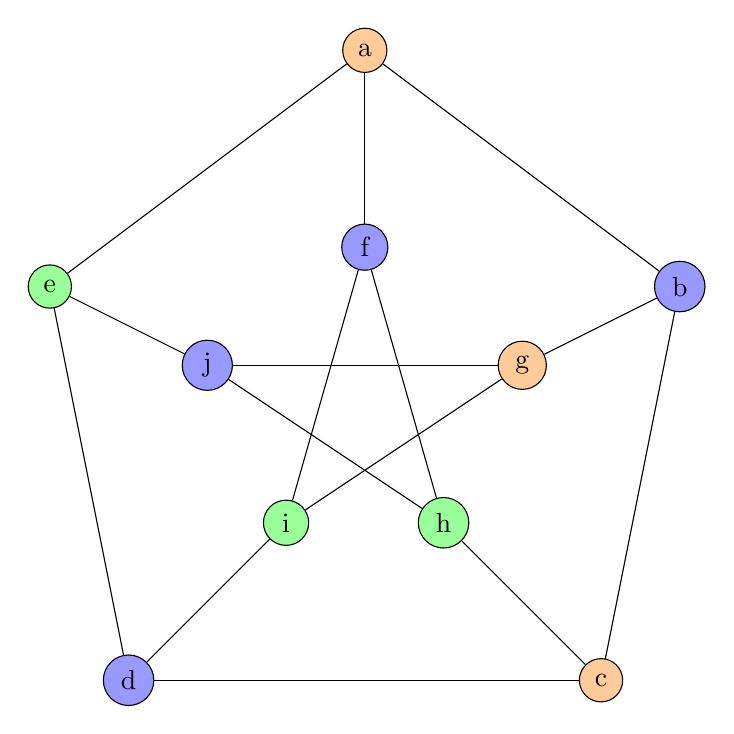
\begin{tikzpicture}[every node/.style={fill=white}, n/.style={circle, draw, fill=#1!40}]
            \node[n={orange}] (a) at (1, 4) {a};
            \node[n={blue}] (b) at (5, 1) {b};
            \node[n={orange}] (c) at (4, -4) {c};
            \node[n={blue}] (d) at (-2, -4) {d};
            \node[n={green}] (e) at (-3, 1) {e};
            \node[n={blue}] (f) at (1, 1.5) {f};
            \node[n={orange}] (g) at (3, 0) {g};
            \node[n={green}] (h) at (2, -2) {h};
            \node[n={green}] (i) at (0, -2) {i};
            \node[n={blue}] (j) at (-1, 0) {j};

            \draw (a) edge (b);
            \draw (a) edge (f);
            \draw (a) edge (e);
            \draw (b) edge (g);
            \draw (b) edge (c);
            \draw (c) edge (h);
            \draw (c) edge (d);
            \draw (d) edge (i);
            \draw (d) edge (e);
            \draw (e) edge (j);
            \draw (f) edge (h);
            \draw (f) edge (i);
            \draw (g) edge (i);
            \draw (g) edge (j);
            \draw (h) edge (j);
        \end{tikzpicture}

        Resultado: 3 cores
    \end{center}
\end{example}

\begin{example}
    \centering
    Cores: \textcolor{orange}{1} \textcolor{blue}{2} \textcolor{green}{3} \textcolor{violet}{4}

    \vspace{\baselineskip}

    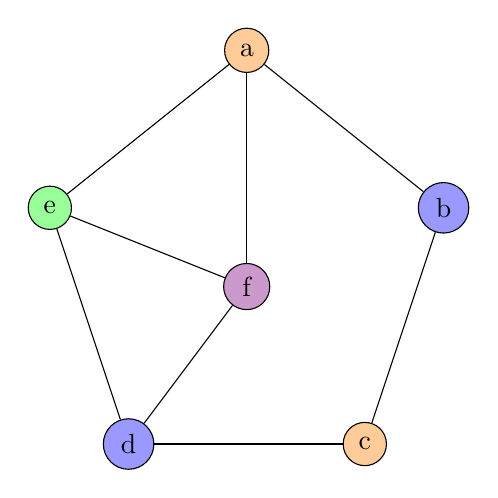
\begin{tikzpicture}[every node/.style={fill=white}, n/.style={circle, draw, fill=#1!40}]
        \node[n={orange}] (a) at (0.5, 2) {a};
        \node[n={blue}] (b) at (3, 0) {b};
        \node[n={orange}] (c) at (2, -3) {c};
        \node[n={blue}] (d) at (-1, -3) {d};
        \node[n={green}] (e) at (-2, 0) {e};
        \node[n={violet}] (f) at (0.5, -1) {f};

        \draw (a) edge (b);
        \draw (a) edge (e);
        \draw (a) edge (f);
        \draw (b) edge (c);
        \draw (c) edge (d);
        \draw (d) edge (e);
        \draw (d) edge (f);
        \draw (e) edge (f);
    \end{tikzpicture}

    Resultado: 4 cores
\end{example}

O problema aqui foi um vértice de maior grau (f). Uma ideia é começar a trabalhar com os vértices de maior grau.

Reordenando, temos:

\begin{example}
    \centering
    Cores: \textcolor{orange}{1} \textcolor{blue}{2} \textcolor{green}{3} \textcolor{violet}{4}

    \vspace{\baselineskip}

    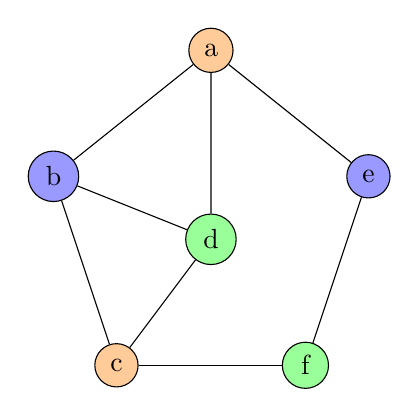
\begin{tikzpicture}[every node/.style={fill=white}, n/.style={circle, draw, fill=#1!40}, scale=.8]
        \node[n={orange}] (a) at (0.5, 2) {a};
        \node[n={blue}] (e) at (3, 0) {e};
        \node[n={green}] (f) at (2, -3) {f};
        \node[n={orange}] (c) at (-1, -3) {c};
        \node[n={blue}] (b) at (-2, 0) {b};
        \node[n={green}] (d) at (0.5, -1) {d};

        \draw (a) edge (b);
        \draw (a) edge (d);
        \draw (a) edge (e);
        \draw (b) edge (c);
        \draw (b) edge (d);
        \draw (c) edge (d);
        \draw (c) edge (f);
        \draw (e) edge (f);
    \end{tikzpicture}

    Resultado: 4 cores
\end{example}

\begin{algorithm}
    \SetAlgoLined
    \SetKwFunction{Coloracao}{ColoracaoGuloso2}
    \Fn{\Coloracao{$G=(V, E)$}}{
        ordene e renomeie os vértices em ordem decrescente de grau\;
        \Para{$v \gets 1$ até $|V|$}{
            seja $i$ a menor cor não presente nos vizinhos de $v$\;
            atribua a cor $i$ a $v$\;
        }
        seja $i_{\mathrm{max}}$ a maior cor utilizazda\;
        \Retorna $i_{\mathrm{max}}$
    }
\end{algorithm}

\section{Corte em grafos}

Um corte é uma bipartição dos vértices de um grafo.

O tamanho do corte é o número de arestas que ``atravessam'' o corte.

\begin{center}
    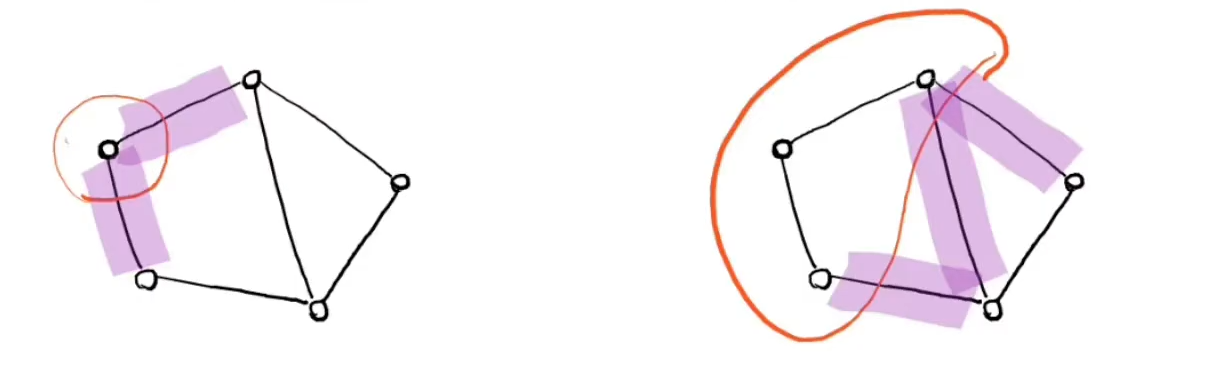
\includegraphics[width=.8\textwidth]{img/arestas_corte.png}
\end{center}

\subsection{Problema do corte máximo}

\begin{itemize}
    \item \textbf{Entrada:} um grafo $G=(V, E)$.
    \item \textbf{Soluções viáveis:} um corte de G, i.e., um conjunto $S$ tal que $\emptyset \neq S \subset V$.
    \item \textbf{Função objetivo:} número de arestas que sai de $S$: $|\delta (S)|$.
    \item \textbf{Objetivo:} encontrar solução de custo máximo.
\end{itemize}

\begin{algorithm}
    \SetAlgoLined
    \SetKwFunction{Corte}{CorteMaximoGuloso}
    \Fn{\Corte{$G=(V, E)$}}{
        $S \gets \emptyset$\;
        $\bar{S} \gets \emptyset$\;
        \Para{$v \in V$}{
            \tcc{Coloca o vértice no conjunto que tem menos vizinhos dele (aumentando o número de arestas que atravessam o corte)}
            \eSe{$|\left\{ (v, u) \in \delta(v): u \in S\right\}| \leq |\left\{ (v, u) \in \delta(v): u \in \bar{S}\right\}|$}{
                $S \gets S \cup \{v\}$\;
            }{
                $\bar{S} \gets \bar{S}\cup\left\{v\right\}$
            }
        }
    }
\end{algorithm}

\begin{example}
    \centering
    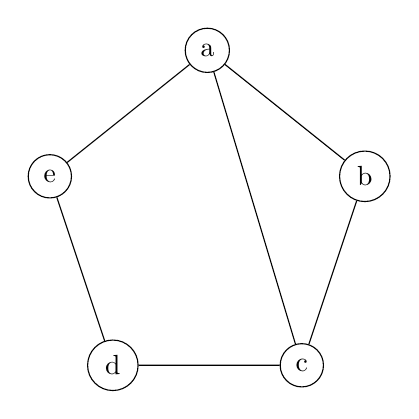
\begin{tikzpicture}[every node/.style={fill=white}, n/.style={circle, draw}, scale=.8]
        \node[n] (a) at (0.5, 2) {a};
        \node[n] (b) at (3, 0) {b};
        \node[n] (c) at (2, -3) {c};
        \node[n] (d) at (-1, -3) {d};
        \node[n] (e) at (-2, 0) {e};

        \draw (a) edge (b);
        \draw (a) edge (c);
        \draw (b) edge (c);
        \draw (c) edge (d);
        \draw (d) edge (e);
        \draw (e) edge (a);
    \end{tikzpicture}

    \vspace{\baselineskip}

    \begin{tikzpicture}[every node/.style={fill=white}, n/.style={circle, draw}]
        \node[n] (a) at (0, 0) {a};
        \node[n] (c) [below=of a] {c};
        \node[n] (e) [below=of c] {e};
        \node[n] (b) at (4, 0) {b};
        \node[n] (d) [below=of b] {d};

        \node[fill=none, draw, ellipse, fit=(a)(c)(e), label=above:$S$] {};
        \node[fill=none, draw, ellipse, fit=(b)(d), label=above:$\bar{S}$] {};

        \draw[thick, red] (a) edge (b);
        \draw (a) edge (c);
        \draw[thick, red] (b) edge (c);
        \draw[thick, red] (c) edge (d);
        \draw[thick, red] (d) edge (e);
        \draw (e) to[out=120, in=-120] (a);
    \end{tikzpicture}

    Solução: 4 arestas
\end{example}

Se atribuir mais cedo os vértices de maior grau (a, c), parece que é melhor. Já que esses vértices ``influenciam mais'' outros.

\begin{example}
    \centering
    \begin{tikzpicture}[every node/.style={fill=white}, n/.style={circle, draw}]
        \node[n] (a) at (0, 0) {a};
        \node[n] (c) at (4, 0) {c};
        \node[n] (b) [below=of a] {b};
        \node[n] (d) [below=of b] {d};
        \node[n] (e) [below=of c] {e};

        \node[fill=none, draw, ellipse, fit=(a)(b)(d), label=above:$S$] {};
        \node[fill=none, draw, ellipse, fit=(c)(e), label=above:$\bar{S}$] {};

        \draw (a) edge (b);
        \draw[thick, red] (a) edge (c);
        \draw[thick, red] (b) edge (c);
        \draw[thick, red] (c) edge (d);
        \draw[thick, red] (d) edge (e);
        \draw[thick, red] (e) edge (a);
    \end{tikzpicture}

    Solução: 5 arestas
\end{example}

\begin{algorithm}
    \SetAlgoLined
    \SetKwFunction{Corte}{CorteMaximoGuloso2}
    \Fn{\Corte{$G=(V, E)$}}{
        $S \gets \emptyset$\;
        $S \gets \emptyset$\;
        $alcancados \gets \left\{ s \right\}$ \tcc*{Inicializa com algum vértice inicial}
        \Para{$v \in alcancados$ \underline{com maior grau}}{
            \eSe{$|\left\{ (v, u) \in \delta(v): u \in S\right\}| \leq |\left\{ (v, u) \in \delta(v): u \in \bar{S}\right\}|$}{
                $S \gets S \cup {v}$\;
                $alcancados \gets alcancados \cup \delta(v)$\;
            }{
                $\bar{S} \gets \bar{S}\cup\left\{v\right\}$\;
                $alcancados \gets alcancados \cup \delta(v)$\;
            }
        }
    }
\end{algorithm}

\section{Problema do Caixeiro Viajante}

\begin{itemize}
    \item \textbf{Entrada:} $G=(V,E)$ e função $\mathrm{w}$ de peso nas arestas.
    \item \textbf{Soluções viáveis:} circuitos hamiltonianos (visitam todos os vértices sem repetição) de $G$.
    \item \textbf{Função objetivo:} soma dos pesos das arestas do circuito.
    \item \textbf{Objetivo:} encontrar um circuito de menor custo.
\end{itemize}

Escolher em cada iteração o vértice com menor custo.

\begin{algorithm}
    \SetAlgoLined
    \SetKwFunction{TSPum}{TSP-Guloso1}
    \Fn{\TSPum{$G=(V, E), \mathrm{w}$}}{
        Seja $C$ um circuito trivial\;
        \Enqto{C não é hamiltoniano}{
            escolha uma aresta $(u, v) \in C$ e um vértice $x \notin C$ que minimizem $\mathrm{w}(u,x) + \mathrm{w}(x,v) - \mathrm{w}(u,v)$\;
            $C \gets C - uv + ux + xv$\;
        }
        \Retorna C
    }
\end{algorithm}

\newpage

\begin{example}
    \begin{center}
        \begin{tikzpicture}[every node/.style={fill=white}, n/.style={circle, draw}]
            \node[n] (a) at (4, 5) {a};
            \node[n] (b) at (0, 0) {b};
            \node[n] (c) at (3, 2) {c};
            \node[n] (d) at (7, 3) {d};
            \node[n] (e) at (5, 0) {e};
            \node[n] (f) at (0, 3) {f};
            \node[n] (g) at (2, -2) {g};

            \draw (a) edge (b);
            \draw (b) edge (c);
            \draw (c) edge (a);
            \draw[dashed] (c) edge (g);
            \draw[dashed] (b) edge (g);
        \end{tikzpicture}
    \end{center}

    Circuito trivial: $\bar{abc}$.

    Vértice que minimiza: $g$, quando inserido entre $b$ e $c$.

    Então, remove a aresta $\bar{bc}$ e adiciona $\bar{bgc}$.

    \begin{center}
        \begin{tikzpicture}[every node/.style={fill=white}, n/.style={circle, draw}]
            \node[n] (a) at (4, 5) {a};
            \node[n] (b) at (0, 0) {b};
            \node[n] (c) at (3, 2) {c};
            \node[n] (d) at (7, 3) {d};
            \node[n] (e) at (5, 0) {e};
            \node[n] (f) at (0, 3) {f};
            \node[n] (g) at (2, -2) {g};

            \draw (a) edge (b);
            \draw (c) edge (a);
            \draw (c) edge (g);
            \draw (b) edge (g);
            \draw[dashed] (g) edge (e);
            \draw[dashed] (e) edge (c);
        \end{tikzpicture}
    \end{center}

    \newpage

    Em seguida, insere o vértice $f$.

    \begin{center}
        \begin{tikzpicture}[every node/.style={fill=white}, n/.style={circle, draw}]
            \node[n] (a) at (4, 5) {a};
            \node[n] (b) at (0, 0) {b};
            \node[n] (c) at (3, 2) {c};
            \node[n] (d) at (7, 3) {d};
            \node[n] (e) at (5, 0) {e};
            \node[n] (f) at (0, 3) {f};
            \node[n] (g) at (2, -2) {g};

            \draw (a) edge (b);
            \draw (c) edge (a);
            \draw (b) edge (g);
            \draw (g) edge (e);
            \draw (e) edge (c);
            \draw[dashed] (f) edge (a);
            \draw[dashed] (f) edge (b);
        \end{tikzpicture}
    \end{center}

    E o vértice $d$ por último.

    \begin{center}
        \begin{tikzpicture}[every node/.style={fill=white}, n/.style={circle, draw}]
            \node[n] (a) at (4, 5) {a};
            \node[n] (b) at (0, 0) {b};
            \node[n] (c) at (3, 2) {c};
            \node[n] (d) at (7, 3) {d};
            \node[n] (e) at (5, 0) {e};
            \node[n] (f) at (0, 3) {f};
            \node[n] (g) at (2, -2) {g};

            \draw (c) edge (a);
            \draw (b) edge (g);
            \draw (g) edge (e);
            \draw (e) edge (c);
            \draw (f) edge (a);
            \draw (f) edge (b);
            \draw[dashed] (a) edge (d);
            \draw[dashed] (d) edge (c);
        \end{tikzpicture}
    \end{center}
\end{example}

\newpage

\subsection{Vértices mais próximos e mais distantes}

Seja $\mathrm{w}(v, C)$ a menor distância de $v$ a um vértice de $C$.

\begin{algorithm}
    \SetAlgoLined
    \SetKwFunction{TSPdois}{TSP-Guloso2}
    \Fn{\TSPdois{$G=(V, E), \mathrm{w}$}}{
        Seja $C$ um circuito trivial\;
        \Enqto{C não é hamiltoniano}{
            escolha um vértice $c \notin C$ que \underline{minimiza} $\mathrm{w}(x, C)$\;
            insira $x$ em C ao lado do vértice mais próximo dele\;
        }
        \Retorna C
    }
\end{algorithm}

É mais fácil calcular a distância de um nó para um conjunto de nós do que calcular o critério de peso de arestas do algoritmo \TSPum.

Para o algoritmo que insere o nó mais distante:

\begin{algorithm}
    \SetAlgoLined
    \SetKwFunction{TSPtres}{TSP-Guloso3}
    \Fn{\TSPtres{$G=(V, E), \mathrm{w}$}}{
        Seja $C$ um circuito trivial, de preferência formado pelos dois vértices mais distantes\;
        \Enqto{C não é hamiltoniano}{
            escolha um vértice $c \notin C$ que \underline{maximiza} $\mathrm{w}(x, C)$\;
            insira $x$ em C ao lado do vértice mais próximo dele\;
        }
        \Retorna C
    }
\end{algorithm}

Esse algoritmo não necessariamente se preocupa em adicionar as arestas de menor peso. Mas é uma heurística e gera uma solução viável.

\subsection{Vizinho mais próximo}

Não mantém um circuito. Constroi um caminho. Ao final cria um circuito ligando as extremidades.

\begin{algorithm}
    \SetAlgoLined
    \SetKwFunction{TSPquatro}{TSP-Guloso4}
    \Fn{\TSPquatro{$G=(V, E), \mathrm{w}$}}{
        Seja $v$ um vértice qualquer\;
        $C \gets (v)$\;
        \Enqto{C não contém todos os vértices}{
            Seja $C = (v_1, \dots , v_i)$\;
            Escolha um vértice $x \notin C$ que \underline{minimiza} $\mathrm{w}(v_i, x)$\;
            Insira $x$ no final de $C$\;
        }
        \Retorna C
    }
\end{algorithm}

O algoritmo \TSPquatro é mais eficiente porque não precisa calcular a distância de cada vértice ao conjunto de vértices (circuito). Calcula apenas a distância com relação a um único vértice $v_i$.